\section{Performances de la Programmation Linéaire Mixte}

\subsection{Modèles indexés par le temps}
\begin{table}[!htb]
  \begin{center}
    \begin{tabular}{|c|cc|cccc|}
      \hline
      \multirow{2}{*}{\#tasks} & \multicolumn{2}{c|}{first sol.}& \multicolumn{4}{c|}{final sol.}\\ 
      \cline{2-7} 
              & time(s) & gap & time & gap &\%solved &  \%opt \\
      \hline 
      \rule[5pt]{0pt}{5pt}
      $10 $& $0,04$ & $10^{75}$ & $0,04$ & $0$ & $100$ & $100$\\ [5pt]
      $20 $& $0,37$ & $10^{75}$ & $0,44$ & $0$ & $100$ & $100$\\ [5pt]
      $25 $& $1,6$ & $10^{75}$ & $1,6$ & $0$ & $100$ & $100$\\ [5pt]
      $30 $& $1,6$ & $10^{75}$ & $1,7$ & $0$ & $100$ & $100$\\ [5pt]
      $60 $& $46$ & $10^{75}$ & $47$ & $0$ & $100$ & $100$\\ 
      \hline 
    \end{tabular}
  \end{center}
  \caption{Résultats du PLNE indexé par le temps pour le \CECSP.}
  \label{tab:TI_CECSP}
\end{table}

\subsection{Modèles à événements}


\subsubsection{Algorithme de séparation pour les inégalités de non
  préemption} 

L'idée principale de la procédure de séparation pour les inégalités de
non préemption est que, pour chaque activité $i$, trouver la coupe à
ajouter au modèle est équivalent à trouver un plus long chemin dans un
certain graphe. Ce graphe orienté et acyclique est défini de la
manière suivante:
\begin{itemize}
\item à chaque événement de l'ensemble $\E^*$=$\E \setminus\{2n\}$,
i.e. $\{1,\dots,2n-1\}$, on fait correpondre un sommet;
\item on ajoute au graphe un source et un puits, indexés
respectivement par $0$ et $2n$. Le graphe est donc composé de $2n+1$
sommets.
\item L'ensemble des arcs est divisé en trois catégories:
  \begin{itemize}
  \item[(i)] les {\it arcs de départ} relient le sommet source $0$ à
chaque sommet $u \in \{1,\dots,2n-3\}$;
  \item[(ii)] les {\it arcs intermédiaires} relient les sommets $u \in
\{1,\dots, 2n-3\}$ aux sommets $v \in \{u+2,\dots,2n-1\}$ et
  \item[(iii)] les {\it arcs terminaux} relient les sommets $u \in
\{3,\dots,2n-1\}$ au sommet puits $2n$;
  \end{itemize}
\end{itemize}

De plus, un coût $cost(u,v)$ est associé à chaque arc $(u,v)$
composant le graphe. Le coût d'un arc de départ est $0$, celui d'un
arc intermédiaire $(u,v)$ est $cost(u,v)= \overline{z}_{i,u} -
\min\{ \overline{z}_{i,\ell}\ :\ \ell= u+1,\dots, v-1\}$ et celui
d'un arc terminal $(u,2n)$ est $\overline{z}_{i,u}$. La construction
de ce graphe est illustré dans l'exemple~\ref{ex:algo_sep}.

\begin{ex}
\label{ex:algo_sep}
Considérons une instance à quatre activités. Le nombre d'événements
$|\E|$ est égale à $8$. Considérons, par exemple, l'activité $1$. Si
nous appliquons la transformation décrite ci-dessus, nous obtenons le
graphe à $9$ sommets et $30$ arcs décrits par la
figure~\ref{fig:algo_sep}. Sur ce graphe, seuls les coûts des arcs
terminaux et des arcs intermédiaires sortant du sommet $2$ sont
représentés. 
\begin{figure}[!htb]
  \centering
  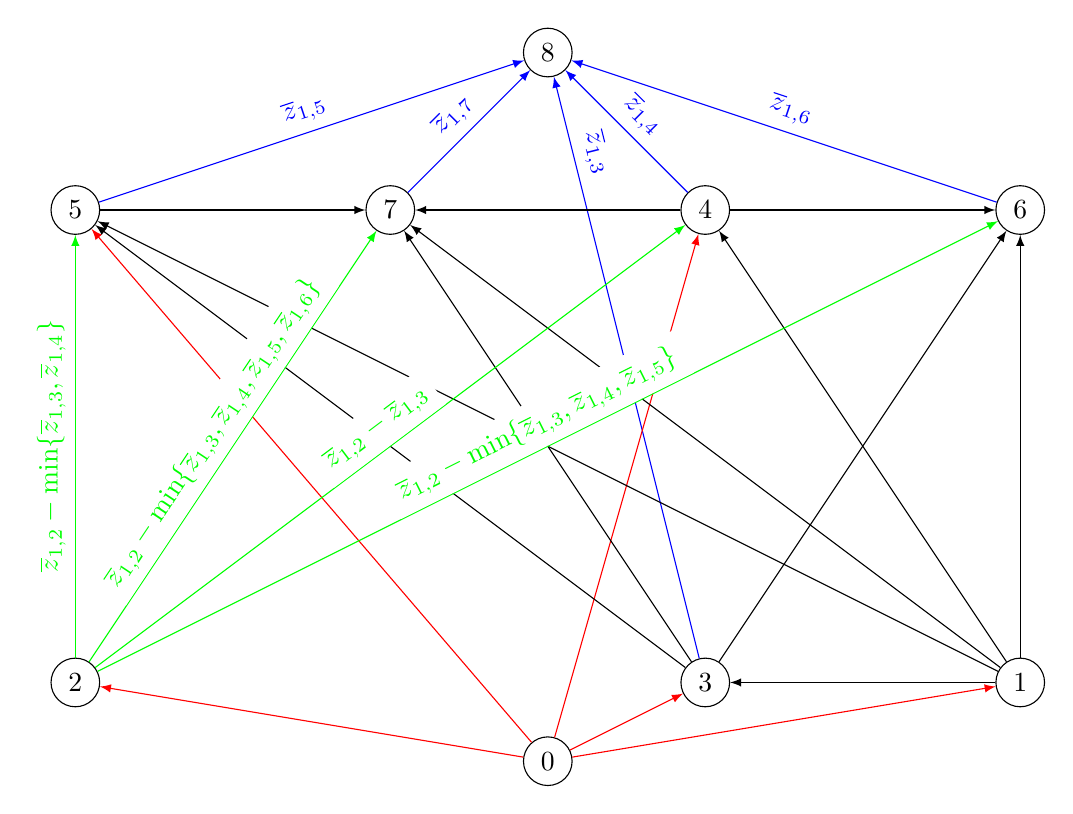
\begin{tikzpicture}
    [  every node/.style={},%
    dot/.style={circle,fill=black,minimum size=4pt,inner sep=0pt,%
      outer sep=-1pt},
    cross/.style={path picture={ 
        \draw
        (path picture bounding box.south east) -- (path picture
        bounding box.north west) (path picture bounding box.south
        west) -- (path picture bounding box.north east); 
      }}]
    \tikzstyle{sommet}=[draw,circle,minimum width=0.5cm]
    \node[sommet] (O) at (0,0) {$0$};
    \node[sommet] (U) at (6,1) {$1$}; 
    \node[sommet] (D) at (-6,1) {$2$}; 
    \node[sommet] (T) at (2,1) {$3$}; 
    \node[sommet] (Q) at (2,7) {$4$}; 
    \node[sommet] (C) at (-6,7) {$5$}; 
    \node[sommet] (Si) at (6,7) {$6$}; 
    \node[sommet] (Se) at (-2,7) {$7$};
    \node[sommet] (H) at (0,9) {$8$};
    
    \draw[->,>=latex,blue] (T) --  node[pos= 0.86,sloped, above] {$
      \overline{z}_{1,3}$} (H) ;
    \draw[->,>=latex,blue] (Q) -- node[sloped,above] {$
      \overline{z}_{1,4}$} (H) ; 
    \draw[->,>=latex,blue] (C) --  node[sloped,above] {$
      \overline{z}_{1,5}$}(H) ; 
    \draw[->,>=latex,blue] (Si) -- node[sloped,above]
    {$ \overline{z}_{1,6}$} (H)  ;
    \draw[->,>=latex,blue] (Se)  -- node[sloped,above] {$
      \overline{z}_{1,7}$} (H) ;
    
    \draw[->,>=latex,red] (O) -- (U);
    \draw[->,>=latex,red] (O) -- (D);
    \draw[->,>=latex,red] (O) -- (T);
    \draw[->,>=latex,red] (O) -- (Q);
    \draw[->,>=latex,red] (O) -- (C);
    
    \draw[->,>=latex] (U) -- (T) ;
    \draw[->,>=latex] (U) -- (Q) ;
    \draw[->,>=latex] (U) -- (C) ;
    \draw[->,>=latex] (U) -- (Si) ;
    \draw[->,>=latex] (U) -- (Se) ;
    
    \draw[->,>=latex] (T) -- (C) ;
    \draw[->,>=latex] (T) -- (Si) ;
    \draw[->,>=latex] (T) -- (Se) ;
    
    \draw[->,>=latex] (Q) -- (Si) ;
    \draw[->,>=latex] (Q) -- (Se) ;
    
    \draw[->,>=latex] (C) -- (Se) ;
    
    \draw[->,>=latex,green] (D) --node[fill=white,sloped,above]
    {$ \overline{z}_{1,2} - \overline{z}_{1,3}$} (Q) ;
    \draw[->,>=latex,green] (D) -- node[fill=white,sloped,above]
    {$ \overline{z}_{1,2} -
      \min\{\overline{z}_{1,3},\overline{z}_{1,4}\}$}(C) ; 
    \draw[->,>=latex,green] (D) -- node[fill=white,sloped,above]
    {$ \overline{z}_{1,2}-
      \min\{\overline{z}_{1,3},\overline{z}_{1,4},\overline{z}_{1,5}\}$}(Si) 
    ; 
    \draw[->,>=latex,green] (D) -- node[fill=white,sloped,above]
    {$
      \overline{z}_{1,2}-\min\{\overline{z}_{1,3},\overline{z}_{1,4},\overline{z}_{1,5},\overline{z}_{1,6}\}$}(Se)
    ; 
    
  \end{tikzpicture}
  \caption{Création du graphe de l'algorithme de séparation pour les
      inégalités de non préemption}
    \label{fig:algo_sep}
  \end{figure}
\end{ex}

Pour séparer un vecteur $\overline{z}_i \in \mathbb{R}^{\E^*}$, nous
calculons un plus long chemin dans le graphe à l'aide de la
programmation dynamique. Pour cela, nous calculons, pour chaque $v \in
\{1,\dots,2n-1\}$, la valeur de du plus long chemin jusqu'à ce somment
$F(v)$ de la manière suivante:
\begin{equation}
  F(v) = \max\{ F(u) + cost (u,v) \ : \ u=1,\dots,v-2 \}
\end{equation}
avec $F(1)=F(2)=0$. 

Puis, on ajoute à ce plus long chemin, la valeur de l'arc servant à
rejoindre le puits. Cela revient à ajouter $\overline{z}_{i,v}$ à
chaque $F(v)$. Si cette valeur est supérieure à celle du
plus long chemin trouvé jusqu'à maintenant, nous remplaçons le plus
long chemin et sa valeur par le nouveau chemin trouvé.

\begin{ex}
Considérons le vecteur $\overline{z}_1$ suivant: $(0,2\, ;\, 0\, ;\,
0,4\, ;\, 0,6\, ;\, 0,6\, ;\, 0\, ;\, 1\, ;\, 0,2)$.

Nous avons $F(1)=F(2)=0$. En effet, l'inégalité devant comporter au moins
trois éléments, $F(1)$ et $F(2)$ ne pourront conduire à une telle
inégalité. La longueur du plus long chemin est initialisée à $0$ et
correpond au chemin vide. De plus,nous avons: 
\begin{itemize}
\item $F(3) =  F(1) + cost (1,3) = F(1) + \overline{z}_{1,1} -
  \overline{z}_{1,2} = 0 + 0,2 - 0= 0,2 $. 
  
  Si nous calculons $F(3)+\overline{z}_{1,3}=0,2+0,4=0,6$. La
  longueur du plus long chemin est donc mise à jour et vaut
  $0,6$. Cette valeur correspondant au chemin $\{1,2,3\}$.
\item $\begin{aligned}[t] 
    F(4) &=  \max \left\{
        \begin{array}{lcl}
          F(1) + cost (1,4) & = & F(1) + \overline{z}_{1,1}  -
                              \min\{\overline{z}_{1,2},\overline{z}_{1,3}\}  \\
          F(2) + cost (2,4) &= & F(2) + \overline{z}_{1,2} -
                              \overline{z}_{1,3}     
        \end{array} \right.\\
    &=  \max \left\{ 
        \begin{array}{lcl}
          0 + 0,2 - 0 &=& 0,2\\
          0 + 0 - 0,4 &= &-0,4 
        \end{array} \right.\\
    &=  0,2
  \end{aligned}$

  Et $F(4)+\overline{z}_{1,4}=0,2+0,6=0,8$. La
  longueur du plus long chemin est donc mise à jour et vaut
  $0,8$. Cette valeur correspondant au chemin $\{1,2,4\}$.

\item $\begin{aligned}[t] 
    F(5) &=  \max \left\{
        \begin{array}{lcl}
          F(1) + cost (1,5) & = & F(1) + \overline{z}_{1,1}  -
                                  \min\{\overline{z}_{1,2},\overline{z}_{1,3},\overline{z}_{1,4}\} 
          \\ 
          F(2) + cost (2,5) &= & F(2) + \overline{z}_{1,2} -
                             \min\{\overline{z}_{1,3}, \overline{z}_{1,4}\}\\
          F(3) + cost (3,5) &= & F(3) + \overline{z}_{1,3} -
                             \overline{z}_{1,4} \\
        \end{array} \right.\\
      &=  \max \left\{ 
        \begin{array}{lcl}
          0 + 0,2 - 0 &=& 0,2 \\
          0 + 0 - 0,4 &= &-0,4 \\
          0,2 + 0.4 - 0,6 &= & 0 \\ 
        \end{array} \right.\\
    &=  0,2
  \end{aligned}$

  Si nous calculons $F(5)+\overline{z}_{1,5}=0,2+0,6=0,8$. Le plus
  long chemin n'est donc pas mis à jour. 

\item $F(6)= 0.2$ et $F(6)+\overline{z}_{1,6}=0,2+0=0,2$. Le plus cours 
  chemin n'es pas mis à jour. 
\item $F(7) = F(4) +\overline{z}_{1,4} -
  \min\{\overline{z}_{1,5},\overline{z}_{1,6}\}= 0,2 + 0,6 - 0 =
  0,8$. De plus, $F(7)+\overline{z}_{1,7}=0,8+1=1,8$. Le longueur du
  plus long est donc mise à jour et vaut $1,8$ et correspond au chemin $\{1,2,4,6,7\}$
\end{itemize}

{\'A} la fin de la procédure, le plus long chemin trouvée est donc
$\{1,2,4,6,7\}$ et l'inégalité correspondante, i.e. celle qui sera
ajoutée au modèle, est:
\[  z_{1,1} - z_{1,2} + z_{1,4} - z_{1,6} + z_{1,7} \le 1  \]
\end{ex}  


\subsubsection{Modèles Start/End}

\subsubsection{Modèles On/Off}







